% !TeX root = ../main.tex
% ========= Anhang ==========================
\section*{Anhang}
\addcontentsline{toc}{section}{Anhang}
\appendix
\renewcommand{\thepage}{\Alph{page}} % Seitenzahlen als A, B, C
\setcounter{page}{1}

% Überschrift eines Anhangs im Stil der BA:  \anhangtitel{A: Titel}
\newcommand{\anhangtitel}[1]{\par\noindent{\large\textbf{Anhang #1}}\par}

\anhangtitel{A: Digitaler Anhang}
\label{page:digitaleAnhang}
\noindent Der digitale Anhang ist auf dem beiliegenden USB-Stick gespeichert.
Folgende Dateien sind in den Ordnern unter den angegebenen Dateipfaden zu finden:
\begin{itemize}
	\item Beschreibung: \\ \texttt{./Anhang(digital)/Ordnername}
\end{itemize}

\newpage
\anhangtitel{B: Weitere Abbildungen}
\label{page:AnhangB}
\begin{figure}[H]
	\centering
	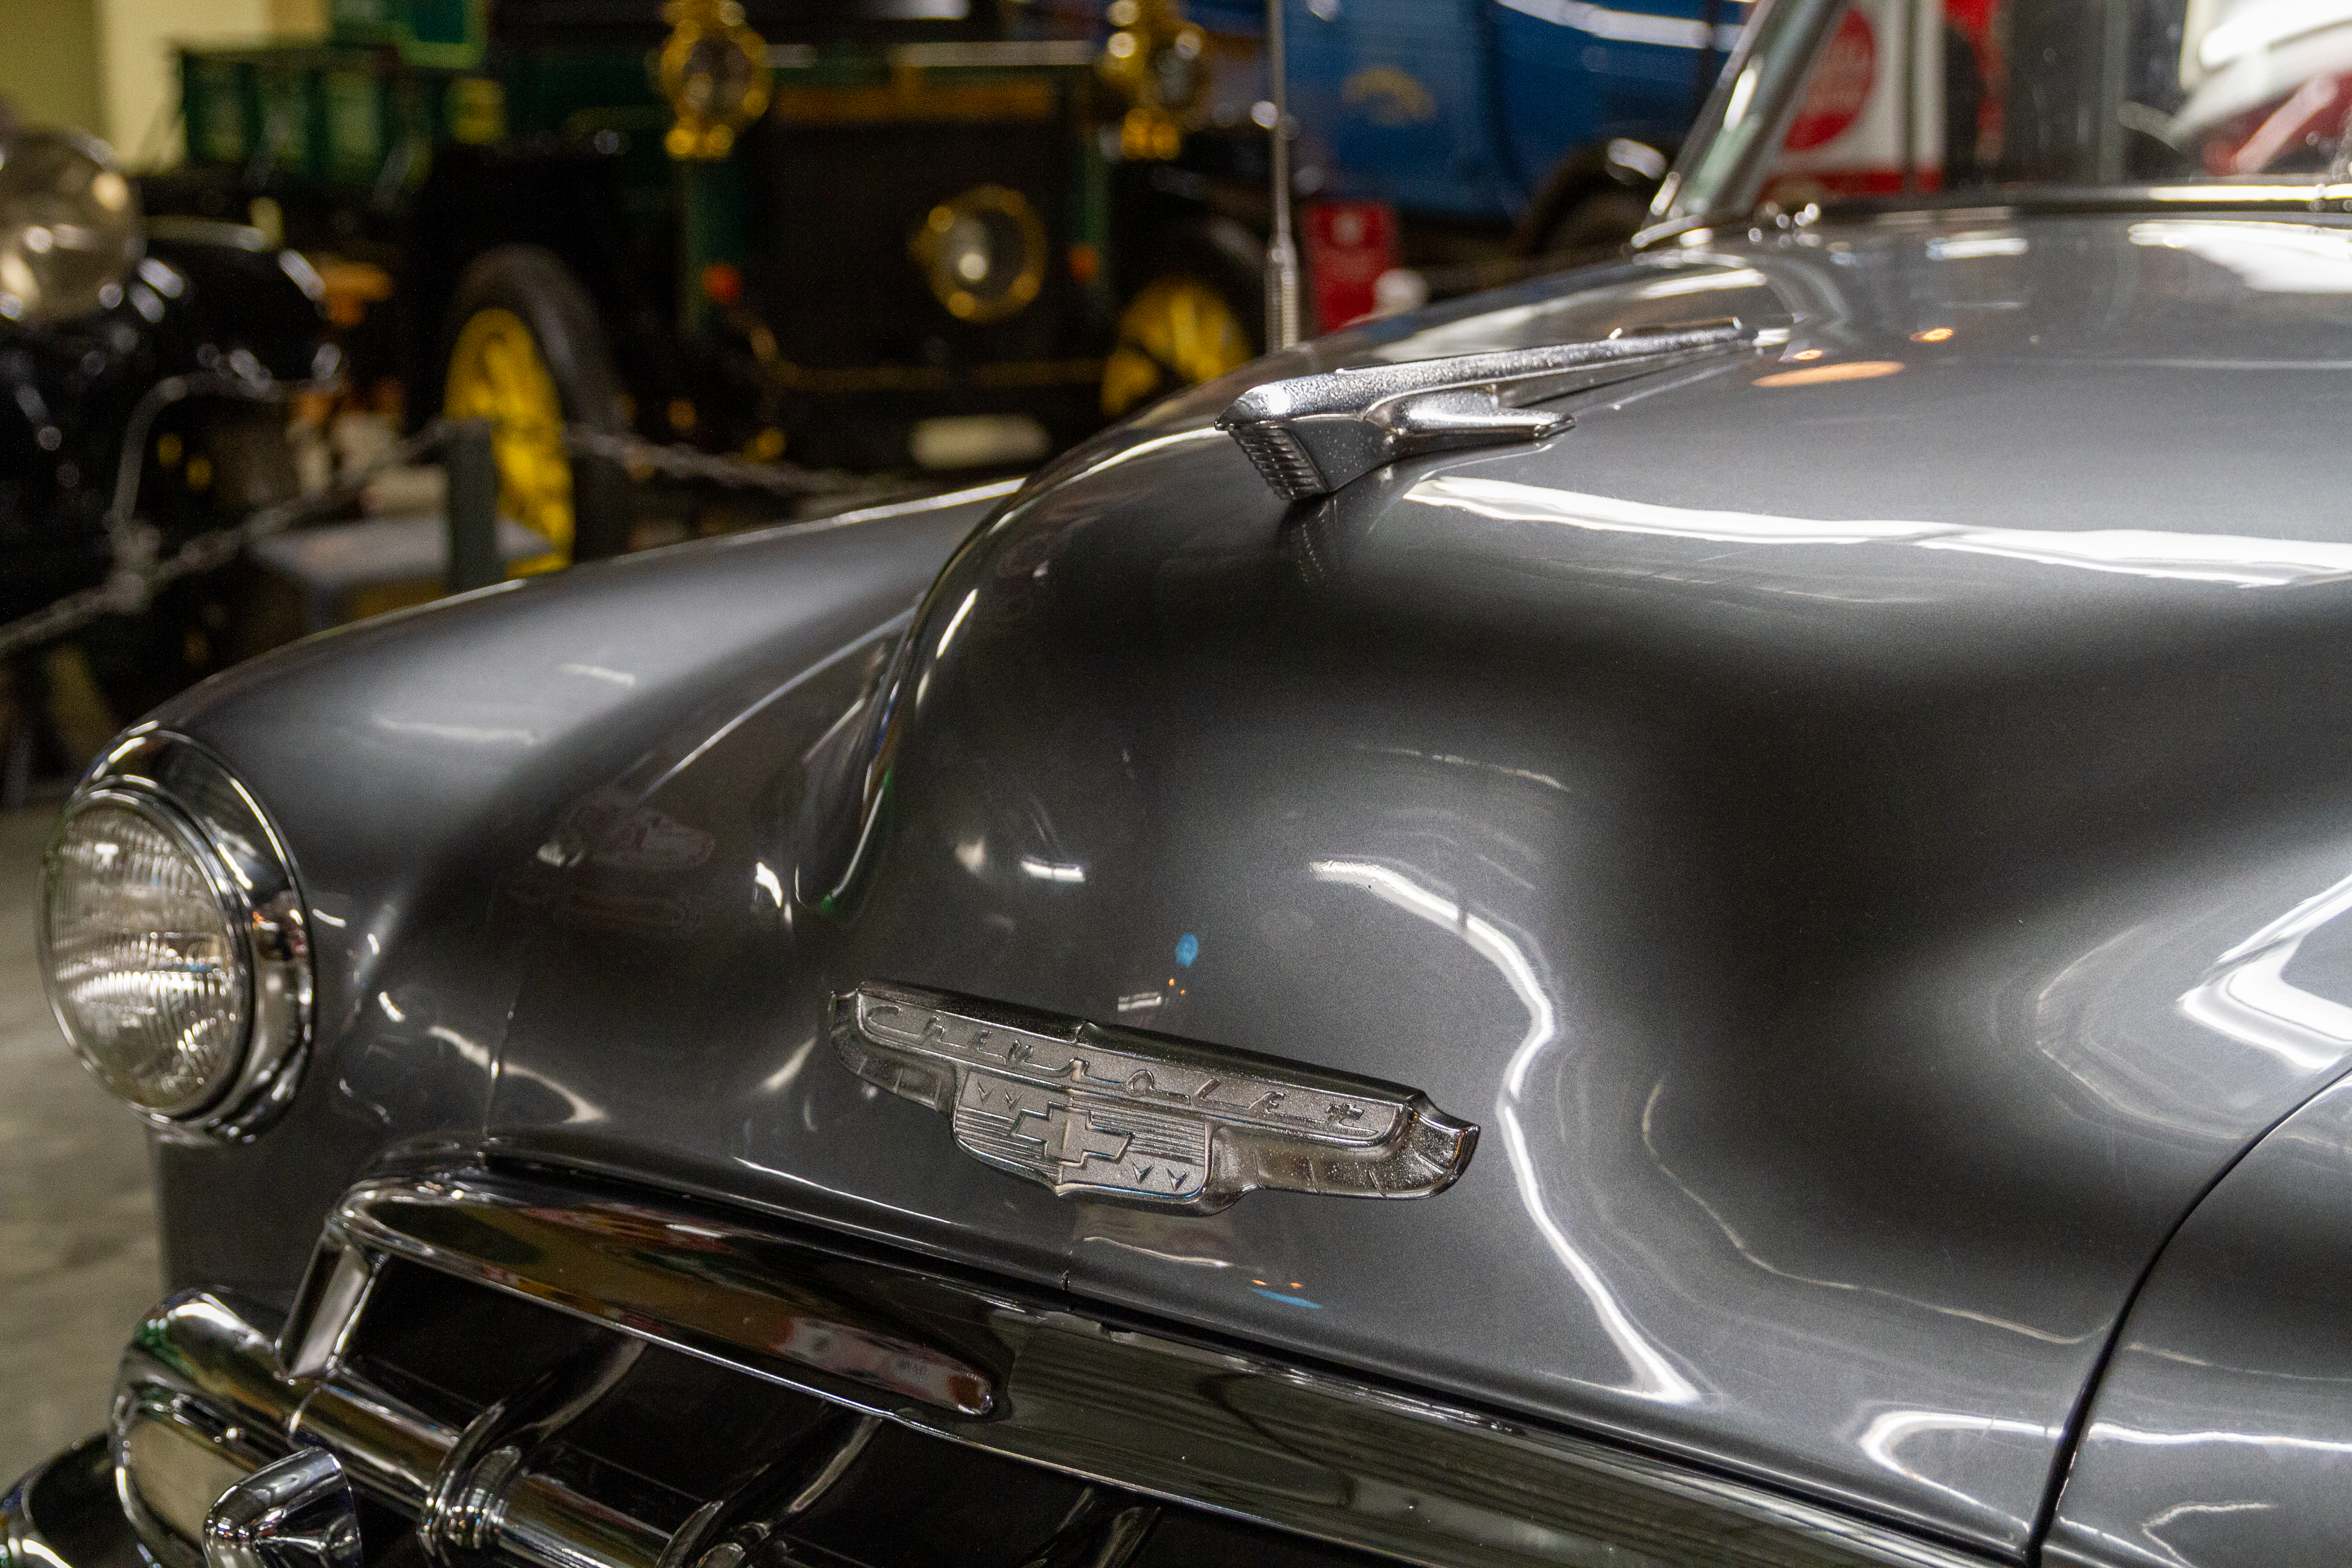
\includegraphics[width=0.6\textwidth]{example-image}
	\caption{Abbildung im Anhang}
	\label{fig:anhang_beispiel}
\end{figure}

% Externe PDF (z. B. Minitab-Bericht) einbinden:
% \newpage
% \includepdf[
%   pages=-,
%   scale=1.0,
%   offset=0 -15,
%   pagecommand={\thispagestyle{plain}\anhangtitel{C: Titel}}
% ]{./abbildungen/Anhang/Bericht.pdf}
